%% BioMed_Central_Tex_Template_v1.06
%%                                      %
%  bmc_article.tex            ver: 1.06 %
%                                       %

%%IMPORTANT: do not delete the first line of this template
%%It must be present to enable the BMC Submission system to
%%recognise this template!!

%%%%%%%%%%%%%%%%%%%%%%%%%%%%%%%%%%%%%%%%%
%%                                     %%
%%  LaTeX template for BioMed Central  %%
%%     journal article submissions     %%
%%                                     %%
%%          <8 June 2012>              %%
%%                                     %%
%%                                     %%
%%%%%%%%%%%%%%%%%%%%%%%%%%%%%%%%%%%%%%%%%


%%%%%%%%%%%%%%%%%%%%%%%%%%%%%%%%%%%%%%%%%%%%%%%%%%%%%%%%%%%%%%%%%%%%%
%%                                                                 %%
%% For instructions on how to fill out this Tex template           %%
%% document please refer to Readme.html and the instructions for   %%
%% authors page on the biomed central website                      %%
%% http://www.biomedcentral.com/info/authors/                      %%
%%                                                                 %%
%% Please do not use \input{...} to include other tex files.       %%
%% Submit your LaTeX manuscript as one .tex document.              %%
%%                                                                 %%
%% All additional figures and files should be attached             %%
%% separately and not embedded in the \TeX\ document itself.       %%
%%                                                                 %%
%% BioMed Central currently use the MikTex distribution of         %%
%% TeX for Windows) of TeX and LaTeX.  This is available from      %%
%% http://www.miktex.org                                           %%
%%                                                                 %%
%%%%%%%%%%%%%%%%%%%%%%%%%%%%%%%%%%%%%%%%%%%%%%%%%%%%%%%%%%%%%%%%%%%%%

%%% additional documentclass options:
%  [doublespacing]
%  [linenumbers]   - put the line numbers on margins

%%% loading packages, author definitions

%\documentclass[twocolumn]{bmcart}% uncomment this for twocolumn layout and comment line below
\documentclass{bmcart}

%%% Load packages
\usepackage{amsthm,amsmath,amssymb}
%\RequirePackage{natbib}
%\RequirePackage[authoryear]{natbib}% uncomment this for author-year bibliography
%\RequirePackage{hyperref}
\usepackage[utf8]{inputenc} %unicode support
%\usepackage[applemac]{inputenc} %applemac support if unicode package fails
%\usepackage[latin1]{inputenc} %UNIX support if unicode package fails
\usepackage{algorithm}
\usepackage{algpseudocode}
\usepackage{multirow}
\usepackage[pass]{geometry}
\usepackage{float}
\newfloat{algorithm}{t}{lop}

%%%%%%%%%%%%%%%%%%%%%%%%%%%%%%%%%%%%%%%%%%%%%%%%%
%%                                             %%
%%  If you wish to display your graphics for   %%
%%  your own use using includegraphic or       %%
%%  includegraphics, then comment out the      %%
%%  following two lines of code.               %%
%%  NB: These line *must* be included when     %%
%%  submitting to BMC.                         %%
%%  All figure files must be submitted as      %%
%%  separate graphics through the BMC          %%
%%  submission process, not included in the    %%
%%  submitted article.                         %%
%%                                             %%
%%%%%%%%%%%%%%%%%%%%%%%%%%%%%%%%%%%%%%%%%%%%%%%%%


%\def\includegraphic{}
%\def\includegraphics{}
\usepackage{graphicx}


%%% Put your definitions there:
\startlocaldefs
\endlocaldefs


%%% Begin ...
\begin{document}

%%% Start of article front matter
\begin{frontmatter}

\begin{fmbox}
\dochead{Research}

%%%%%%%%%%%%%%%%%%%%%%%%%%%%%%%%%%%%%%%%%%%%%%
%%                                          %%
%% Enter the title of your article here     %%
%%                                          %%
%%%%%%%%%%%%%%%%%%%%%%%%%%%%%%%%%%%%%%%%%%%%%%

\title{Machine learning-based analysis of the relationship between bone density and drinking patterns of primates}

%%%%%%%%%%%%%%%%%%%%%%%%%%%%%%%%%%%%%%%%%%%%%%
%%                                          %%
%% Enter the authors here                   %%
%%                                          %%
%% Specify information, if available,       %%
%% in the form:                             %%
%%   <key>={<id1>,<id2>}                    %%
%%   <key>=                                 %%
%% Comment or delete the keys which are     %%
%% not used. Repeat \author command as much %%
%% as required.                             %%
%%                                          %%
%%%%%%%%%%%%%%%%%%%%%%%%%%%%%%%%%%%%%%%%%%%%%%

\author[
   addressref={aff1},                   % id's of addresses, \emph{e.g.} {aff1,aff2}
   corref={aff1},                       % id of corresponding address, if any
%   noteref={n1},                        % id's of article notes, if any
   email={Pablo.Rivas@Marist.edu}   % email address
]{\inits{P}\fnm{Pablo} \snm{Rivas}}
\author[
   addressref={aff2},
   email={urszula.iwaniec@oregonstate.edu}
]{\inits{UI}\fnm{Urszula} \snm{Iwaniec}}
\author[
   addressref={aff3},
   email={grantka@ohsu.edu}
]{\inits{KA}\fnm{Kathleen A.} \snm{Grant}}
\author[
   addressref={aff4},
   email={Erich\_Baker@Baylor.edu}
]{\inits{E}\fnm{Erich} \snm{Baker}}

%%%%%%%%%%%%%%%%%%%%%%%%%%%%%%%%%%%%%%%%%%%%%%
%%                                          %%
%% Enter the authors' addresses here        %%
%%                                          %%
%% Repeat \address commands as much as      %%
%% required.                                %%
%%                                          %%
%%%%%%%%%%%%%%%%%%%%%%%%%%%%%%%%%%%%%%%%%%%%%%

\address[id=aff1]{%                           % unique id
  \orgname{School of Computer Science and Mathematics, Marist College}, % university, etc
  \street{3399 North Road},                     %
  \postcode{12601}                                % post or zip code
  \city{Poughkeepsie, NY},                              % city
  \cny{USA}                                    % country
}
\address[id=aff2]{%
  \orgname{College of Public Health and Human Sciences, Oregon State University},
  \street{108 Milam Hall},
  \postcode{97331}
  \city{Corvallis, OR},
  \cny{USA}
}
\address[id=aff3]{%
  \orgname{Department of Behavioral Neuroscience, Oregon Health and Science University},
  \street{3181 SW Sam Jackson Park Rd},
  \postcode{97239}
  \city{Portland, OR},
  \cny{USA}
}
\address[id=aff4]{%
  \orgname{Department of Computer Science, Baylor University},
  \street{One Bear Place \#97356},
  \postcode{76798}
  \city{Waco, TX},
  \cny{USA}
}

%%%%%%%%%%%%%%%%%%%%%%%%%%%%%%%%%%%%%%%%%%%%%%
%%                                          %%
%% Enter short notes here                   %%
%%                                          %%
%% Short notes will be after addresses      %%
%% on first page.                           %%
%%                                          %%
%%%%%%%%%%%%%%%%%%%%%%%%%%%%%%%%%%%%%%%%%%%%%%

\begin{artnotes}
%\note{Sample of title note}     % note to the article
%\note[id=n1]{Equal contributor} % note, connected to author
\end{artnotes}

\end{fmbox}% comment this for two column layout

%%%%%%%%%%%%%%%%%%%%%%%%%%%%%%%%%%%%%%%%%%%%%%
%%                                          %%
%% The Abstract begins here                 %%
%%                                          %%
%% Please refer to the Instructions for     %%
%% authors on http://www.biomedcentral.com  %%
%% and include the section headings         %%
%% accordingly for your article type.       %%
%%                                          %%
%%%%%%%%%%%%%%%%%%%%%%%%%%%%%%%%%%%%%%%%%%%%%%

\begin{abstractbox}

\begin{abstract} % abstract
\parttitle{Background} %if any
Alcohol use disorders (AUDs) represent one of the largest causes of death in the
world. More research is needed to understand of the underlying relationships between diverse
factors contributing to AUDs, which may lead to models for prevention and treatment of
alcohol abuse-related disease, such as bone damage. 

\parttitle{Methods} %if any
We use a machine learning techniques to investigate the relevance of
features from a dataset of monkeys that were subject to an experiment where
they self-administered alcohol. We use support vector machines for regression
to predict bone mineral density from variables related to drinking and we rank
all the features and sets of features to determine which features and which
sets of features are more predictive of bone damage.

\parttitle{Results} %if any
Empirical evidence suggests that the age at which the monkeys were 
intoxicated for the first time is one of the
best predictors along with information about the maximum bout volume and the
percentage of ethanol consumed during a period of two hours in which the
monkeys had unlimited access to alcohol. We
proved that such features are the best predictors 
using Friedman's test and Nemenji's test with confidence of
$\alpha=0.05$ and $\alpha=0.01$ respectively. 


\parttitle{Conclusion} %if any
Machine learning strategies can successfully inform about the relationship
between bone mineral density and alcohol consumption data from primates.
Specifically, the investigation of which features are more relevant, both by
themselves and as sets, providing the means for better 
understanding the contribution of
some variables over others in the modeling of AUDs.
\end{abstract}

%%%%%%%%%%%%%%%%%%%%%%%%%%%%%%%%%%%%%%%%%%%%%%
%%                                          %%
%% The keywords begin here                  %%
%%                                          %%
%% Put each keyword in separate \kwd{}.     %%
%%                                          %%
%%%%%%%%%%%%%%%%%%%%%%%%%%%%%%%%%%%%%%%%%%%%%%

\begin{keyword}
\kwd{alcohol use disorders}
\kwd{machine learning}
\kwd{support vector regression}
\kwd{forward selection}
\kwd{backward selection}
\kwd{relevance feature ranking}
\end{keyword}

% MSC classifications codes, if any
%\begin{keyword}[class=AMS]
%\kwd[Primary ]{}
%\kwd{}
%\kwd[; secondary ]{}
%\end{keyword}

\end{abstractbox}
%
%\end{fmbox}% uncomment this for twcolumn layout

\end{frontmatter}

%%%%%%%%%%%%%%%%%%%%%%%%%%%%%%%%%%%%%%%%%%%%%%
%%                                          %%
%% The Main Body begins here                %%
%%                                          %%
%% Please refer to the instructions for     %%
%% authors on:                              %%
%% http://www.biomedcentral.com/info/authors%%
%% and include the section headings         %%
%% accordingly for your article type.       %%
%%                                          %%
%% See the Results and Discussion section   %%
%% for details on how to create sub-sections%%
%%                                          %%
%% use \cite{...} to cite references        %%
%%  \cite{koon} and                         %%
%%  \cite{oreg,khar,zvai,xjon,schn,pond}    %%
%%  \nocite{smith,marg,hunn,advi,koha,mouse}%%
%%                                          %%
%%%%%%%%%%%%%%%%%%%%%%%%%%%%%%%%%%%%%%%%%%%%%%

%%%%%%%%%%%%%%%%%%%%%%%%% start of article main body
% <put your article body there>

%%%%%%%%%%%%%%%%
%% Background %%
%%
\section*{Background}

The mining and modeling of biological data is not trivial either in cases
where the data is abundant or scarce. This creates problems of large-scale learning
and analysis of Big Data as well as feature selection in smaller-scale problems
where there is risk of finding under-determined solutions or ill-posed models.
Biological data varies greatly depending of the field of study since
measurements and meaning of the attributes are extremely different. Our
research deals with the specific problem of data analysis for alcohol drinking
pattern in primates as we aim to provide a better understanding of the
different aspects that model alcohol use disorders (AUDs).

Currently, AUDs is a worldwide issue that has been officially presented as 
one of the most deadly disorders
in the United States \cite{mokdad2004actual}. Recent studies indicate that
there is a clear increase in the number of AUD cases
\cite{grant2004prevalence}, and we need a better understanding of all the
influencing factors in AUDs, such as sex, income, and other disorders that are
concurrently pathological \cite{grant2015epidemiology}. To alleviate the need of
understanding all the variables that play an important role in AUDs we
developed a non-human primate (NHP) 
macaque model of oral alcohol self-administration that has identified 
a range of daily ethanol intakes that encompass categorical levels 
of drinking severity, \emph{i.e.}, Low Drinkers (LD), Binge Drinkers 
(BD), Heavy Drinkers (HD), and Very Heaver Drinkers (VHD)
\cite{baker2014chronic}. These categories are a reflection of AUDs severity, especially
with respect to HD and VHD categories since they are associated with problems
of dependence and other brain pathologies
\cite{kroenke2014monkeys,chen2011striatal,siciliano2015voluntary}. However,
such categories do not prescribe by themselves all that is necessary for
modeling AUDs. Therefore, the analysis of other factors using machine learning
techniques is ultimately important.

In this research we report on the study of drinking patterns of monkeys that
were subject to a process of alcohol self-administration. The protocol followed
has been established previously \cite{grant2008drinking}, and it is known as
``schedule-induced polydipsia''. From this induction protocol we recorded data for
further analysis. In particular, we explore different feature ranking strategies
that allow us to understand non-trivial associations using machine learning
algorithms. We make use of correlation, entropy, density, and forward-backward
selection of features as indicators of the relationship between features and
their relevance in the problem of modeling bone damage in primates \cite{guyon2008feature}.  

Using support vector machines for regression as a control model for prediction
\cite{rivas2014algorithm}, we rank
the feature selection methods to further identify which features are more
predictive of bone mineral density (BMD). The study of the relationship between
alcohol consumption patterns and BMD is important for the understanding of the
underlying system that causes permanent bone damage. In this paper we will show
that the amount of alcohol consumed in a period of two hours of open access to
ethanol is one of the most determining factors of BMD 
in monkeys that were intoxicated early in life.
 

\section*{Methods}
\subsection*{Primate Subjects}
We studied the post-mortem BMD of primates from the
Oregon  National  Primate  Research Center  (ONPRC)
to determine which parameters of alcohol consumption are more predictive of BMD
values. We considered a total of 68 monkeys out of which 14 are females and 54
are males. They are of two species known as Cynomolgus and Rhesus. Table
\ref{tbl:cohorts} summarizes the information about the monkeys of each cohort. Our 
study consists of nine cohorts in total. The table also indicates the drinking
category count for each cohort. Most monkeys fall into the category of low
drinkers (LDs). Note, however, that not all cohorts had a category assigned to
them, as is the case of cohort ``INIA Cyno 8'', which, at the moment of this
research, has partial drinking information. Nonetheless, there are other
alcohol consumption parameters available that are considered further.

\begin{table}[t]
\caption{Summary of monkey cohorts. This study includes two species 
of primates: Cynomolgus and Rhesus. Most monkeys are males and low drinkers. 
Drinking category was not available for some Cynomolgus monkeys at the date of
this research.}
\label{tbl:cohorts}
      \begin{tabular}{lccccccc}
        \hline
   Cohort Name &  Total &  Females &  Males &  BD &  LD &  HD &  VHD \\ \hline
   INIA Cyno 2 &     12 &        0 &     12 &   0 &  10 &   0 &    1 \\
INIA Rhesus 7a &      8 &        0 &      8 &   1 &   3 &   2 &    2 \\
   INIA Cyno 9 &     11 &        0 &     11 &   0 &   6 &   2 &    0 \\
   INIA Cyno 8 &      3 &        3 &      0 &   0 &   0 &   0 &    0 \\
INIA Rhesus 7b &      5 &        0 &      5 &   1 &   3 &   1 &    0 \\
 INIA Rhesus 4 &     10 &        0 &     10 &   4 &   5 &   1 &    0 \\
 INIA Rhesus 5 &      8 &        0 &      8 &   1 &   0 &   3 &    4 \\
INIA Rhesus 6a &      6 &        6 &      0 &   0 &   0 &   0 &    6 \\
INIA Rhesus 6b &      5 &        5 &      0 &   0 &   3 &   1 &    1 \\ \hline
         Total &     68 &       14 &     54 &   7 &  30 &  10 &   14 \\ \hline
      \end{tabular}
\end{table}

With partially available drinking categorical data the task of directly
associating BMD with a specific drinking category is cumbersome. Figure
\ref{fig:bmdsexcat} depicts the average BMD of monkeys broken down by gender
and drinking category. The figure suggests no apparent BMD difference between
drinking categories. Although it may seem that low drinking females have more
BMD when compared to high drinking females, the standard deviation, indicated
in the figure, suggests that such conclusion could be misleading.

\begin{figure}[t]
    \caption{\csentence{Bone mineral density by drinking category and sex.}
             There is no significant difference between drinking categories
             or sex. It may seem that high drinking females have lower bone 
             density compared to low drinking ones; however, the standard
	     deviation indicator makes such assumption unreliable. The
             horizontal axis shows the following drinking categories: 
             low drinker (LD), binge drinker (BD), heavy drinker (HD), 
             and very heavy drinker (VHD). There are no females reported as
             BDs.}
\label{fig:bmdsexcat}
    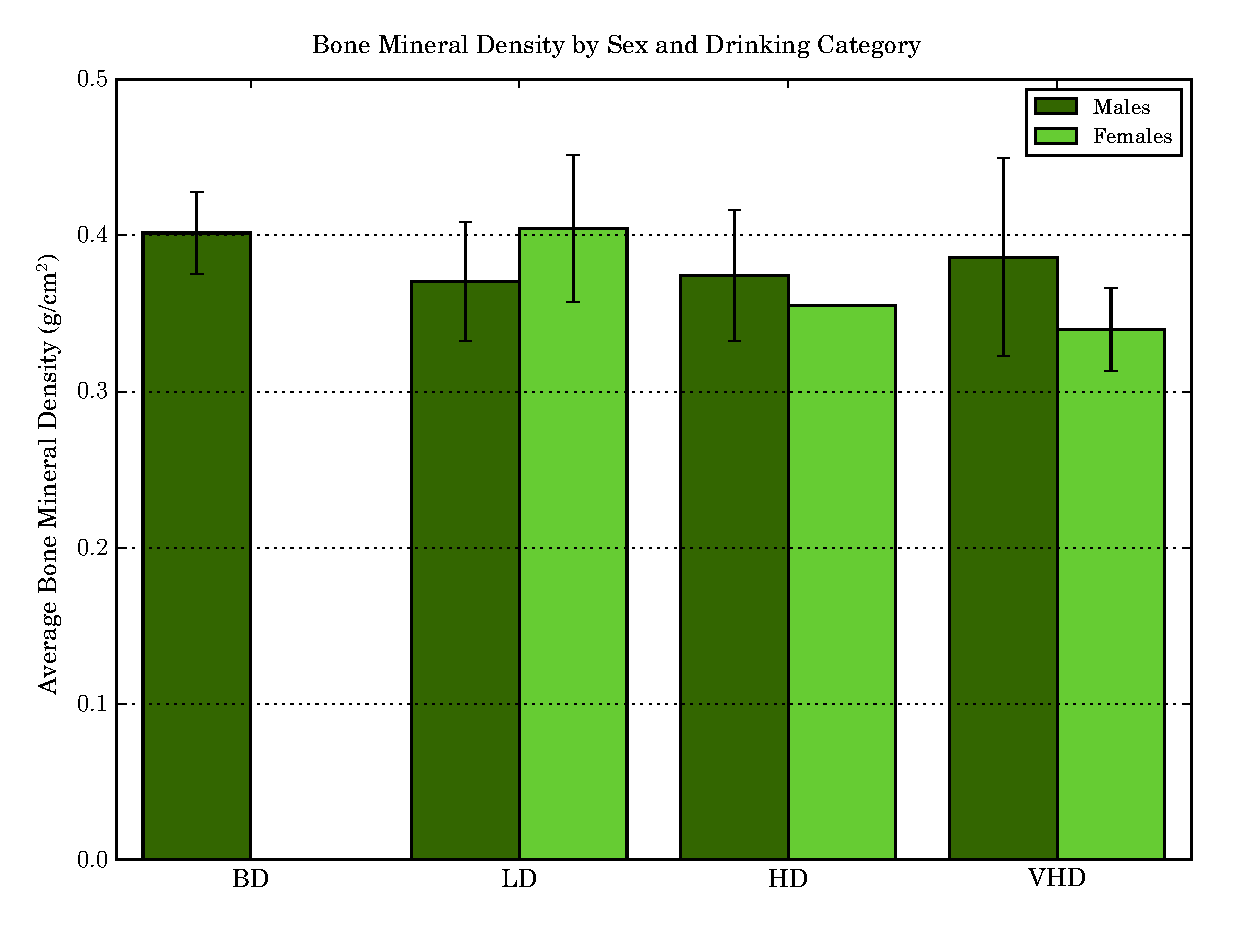
\includegraphics[width=0.9\textwidth]{data_b_c_s_bmd.eps}
\end{figure}

The next step is to consider other factors that could be associated with BMD.
This research considers not only sex as a possible determining factor of BMD, 
but it also considers investigating ethanol (EtOh) consumption patterns
in sets that are potentially predictive of BMD. The EtOh consumption data comes
from experiments carried at the ONPRC, which are described next.

\subsection*{Housing and Development}

Pedigreed monkeys were born into a population remaining with their mothers
until they were about two years old and completely independent from their
mothers for survival. After that, the monkeys were part of an experiment
designed to study alcohol consumption and their physiological and biological 
effects. Monkeys were continually housed at the ONPRC and entered into an internal
housing laboratory with individual caging at
least three months prior to the onset of ethanol self-administration according
to established protocols \cite{daunais2014monkey}. The age of onset is defined as
the number of days a monkey has lived until their blood ethanol concentration 
(BEC) is greater than 80 mg/dl \cite{li2007alcohol,dawson2008age}.

Some monkeys are members of the Cynomolgus cohort that, in our previous
research \cite{grant2008drinking}, have been identified as chronic heavy drinkers. 
The age of the monkeys in this experiment varies starting from late
adolescence to early middle age. Our recent findings indicate that age was also
a contributing factor for chronic levels of alcohol intake of the Cynomolgus
cohort \cite{daunais2014monkey}.

The preparation for the ethanol consumption study involved the setting of four
individual cages belonging to a single rack, two above and two below in a
horizontal arrangement. Each individual cage had a panel providing the means
for drinking water or alcohol. For the comfort of heavier monkeys, over 10kg, they
were allowed to occupy two horizontal cages but only one drinking panel was
available. A single cohort occupied a single space using racks as necessary,
providing visual and auditory contact with other monkeys. In the case of females,
tactile access was available by permitting entry to a common area two hours a
day, which was made by removing the horizontal divisory barrier between two
horizontally adjacent cages. In the case of males,
tactile interchange was available since adjacent males were accessible through
groom panel inserts in the common wall of the cage. Details of the panels for
drinking are described in full in our previous research
\cite{vivian2001induction,grant2008drinking}. The function of such panels is
described next.


\subsection*{Ethanol Self-Administration}

In this study we had panels permanently affixed to individual cages allowing 
access to food and fluid.
We collected data every time food or fluid was self-administered by monkeys.
During our research we followed a previously established procedure that we
defined as ``schedule-induced polydipsia'' \cite{grant2008drinking}, which we
will refer to as ``induction'', for short. In such process we induced monkeys 
to self-administer 4 w/v (\%) EtOh in water. The defining feature of the
induction procedure is a monotonic increase in the maximum volume of EtOh
allowed for consumption. This increase occurs every 30 days in the following
order: 0 g/kg/d, which is a volume of water equivalent to 1.5 g/kg of EtOH, then
to 0.5 g/kg/d, next to 1.0 g/kg/d, and finally to 1.5 g/kg/d. In this manner,
all monkeys drank to levels that saturated metabolic capacity elevating
their BEC over 50 mg/dl. 

After the 30th session of 1.5 g/kg EtOH under induction the monkeys had
concurrent access to 4 w/v (\%) EtOh and a 22 h/d ``open-access'' to water and food
in the form of 1g of banana flavored pellets (Noyes), provided at
least three times a day during meals, and at least two hours apart with the first
meal provided at the beginning of the session. The open-access phase comprises
12 months. Blood ethanol concentration levels were measured every fifth day 30, 60, and 90
minutes after the beginning of the induction sessions and approximately every
fifth day seven hours after the start of the open-access sessions, which
corresponds to the onset of the dark phase of the 11 hour day and 13 hour night 
diurnal cycle.


\subsection*{Computational Resources for Analysis}

All computations were executed on MATRR’s web and database servers. These are
twin dedicated computers each running four Intel Xeon E5620 processors at 2.4
GHz, with four cores per processor, \emph{i.e.}, a total of 16 cores per server.
Each server has 47 GiB of random access memory (RAM) and 1.7 TiB of disk space in
a redundant array of independent disks (RAID) configuration. Web services use
Django's object-relational mapping (ORM) for database access. We carried out
all statistical analysis and data processing using Pandas, NumPy,
and SciPy, which are packages for the Python programming language. For all
machine learning algorithms we used Python’s Scikit-Learn package. Graphical
results, such as the figures in this paper, were produced with the Python 
package called Matplotlib. 


\subsection*{Drinking Features for Analysis}

In our research we studied five factors contributing to the correct prediction
of BMD. From such factors, also known as attributes, we produced a total of 
14 attributes. In machine learning research, we call this attributes
``features''. All 14 features are explained by groups in the next paragraphs.

\subsubsection*{Drinking Category}
Each monkey can be classified to belong to one of the following four
categories, if enough data is available: low drinker (LD), binge drinker (BD),
heavy drinker (HD), and very heavy drinker (VHD). We provide specific details
of the defining criteria for each category in \cite{baker2014chronic}. The data
collected has monkeys categorized as follows: BDs: 11.5\%, LDs: 49.2\%, HDs:
16.4\%, and VHDs: 22.94\%. 

\subsubsection*{Sex}
This feature represents the sex of each monkey. The distribution of the monkeys
in this feature is as follows: Females: 20.6\% and Males: 79.4\%.

\subsubsection*{Age at First Intoxication (in Days)}
The number of days a monkey has lived until the first time its BEC level is
greater than 80 mg/dl describes the age at onset or ``age at first
intoxication''. In this research the average age at first intoxication is $\mu =
2292$ days with a standard deviation of $\sigma = 510$ days.i The age at first
intoxication is often associated with the drinking category of monkeys
\cite{alex2015}.

\subsubsection*{Maximum Bout Volume (in mL)}
The volume in mL of each bout of EtOh a monkey drinks is recorded and organized
by session. One session is equivalent to one day. The volume of the maximum
bout per each session is available per monkey. We particularly focus in the
maximum bout volume that occurs during the first 120 minutes after monkeys had
open-access to EtOh. The overall average maximum bout volume is $\mu =
0.728$ mL with a standard deviation of $\sigma = 0.365$ mL.

From this data we extracted the following five features per monkey for the
first 120 minutes of all sessions: 
a) average maximum bout volume ($\mu$), b) standard deviation of the maximum bout 
volume ($\sigma$), c) median of the maximum bout volume, d) maximum of the maximum bout
volume ($\max$), and e) minimum of the maximum bout volume ($\min$).

\subsubsection*{EtOh During Induction (in \%)}
During the period of induction, explained earlier, monkeys are exposed to
limited amounts of EtOh. Such limits decrease gradually until the monkeys pass
the period of induction to full unrestricted access. However, during the period
of induction we recorded, in percentage, the amount of EtOh the monkeys ingest
out of what they are allowed to drink.

Percentages of EtOh during induction are available per monkey and per session.
From all this data we extract the following six features: a)
average \% of EtOh during induction ($\mu$), b) median \% of EtOh during
induction, c) total sum of the \% of EtOh during induction ($\Sigma$), d)
standard deviation of the \% of EtOh during induction ($\sigma$), e)
minimum \% of EtOh during induction ($\min$), and f) maximum \% of EtOh during
induction ($\max$).

\subsubsection*{Bone Mineral Density (in g/cm$^2$)}
This feature is the object of our study. In machine learning this feature is
called the target. Since the target variable is not a categorical one,
regression algorithms are preferred for analysis that go beyond basic
statistical examination.  

The average BMD is $\mu = 0.376$ g/cm$^2$ and the standard deviation is $\sigma =
0.049$g/cm$^2$. In the following paragraphs we explain the methodologies we use to
analyze the importance or contribution of the above features in predicting BMD
or in finding the parameters of a machine learning model predictive of BMD.


\subsection*{Estimation of Importance and Feature Ranking}

In data mining and machine learning in general, researchers aim to have models
that are computationally inexpensive and robust. One factor that reduces the
risk of poor performance and high complexity is the selection of a set of
features that together provide the best way of modeling the desired output. The
most popular way of selecting ``good'' features is known as ``feature ranking''
\cite{guyon2008feature}.

Feature ranking can be done in an individual manner where each feature is
evaluated by its relevance in predicting the target data. Usually,
individual relevance ranking yields good results, especially when the
features are independent and identically distributed (IID). When the data is
not IID, there is a risk of discarding features that, if combined with others,
may have greater relevance.

In this research we explored methods that evaluate features independently and
in sets of features to determine their relevance. The determination of their
relevance will give us insight as to which features are associated with BMD,
providing a better understanding of how alcohol consumption relates to BMD.

The next paragraphs briefly describe two methods for individual relevance
ranking, Pearson correlation, entropy, and density; and also three methods for combined
relevance ranking, which are based on the well-known 
support vector machines for regression (SVRs) \cite{rivas2014algorithm}.

\subsubsection*{Pearson Correlation}

Let $\mathbf{x}$ be a feature vector of dimension $n$, $\mathbf{x}=[x_1, x_2,
\dots, x_n]$, where $n=14$ is the total number of features in the original
dataset. A single feature vector $\mathbf{x}$ is also known as an observation. 
Let $y$ be a the target, or desired output, of the learning model
and that is paired in a tuple with a single feature vector $\mathbf{x}$. Then,
we can define the dataset as $\mathcal{D}=\left\{ \mathbf{x}_i, y_i
\right\}_{i=1}^m$, where $m$ is the total number of samples. It is important to
remark that feature selection becomes crucial for cases where $m<n$, or when
the dataset is small in general.

The Pearson correlation coefficient, $C$ is a classical measure of
relevance for individual feature ranking. If we define $\mathbf{x}_j$ as a
vector that contains all the observations corresponding to the individual
feature $j$, then the Pearson correlation coefficient of feature $j$ with
respect to the target vector $\mathbf{y}=[y_1, y2_, \dots, y_m]$ is defined 
by the following equation:
\begin{equation}
C(j) = \frac{\left| \sum_{i=1}^m (x_{i,j} - \bar{x}_j) (y_i -\bar{y})
\right|}{\sqrt{\sum_{i=1}^m (x_{i,j} - \bar{x}_j)^2 \sum_{i=1}^m(y_i
-\bar{y})^2}} , 
\end{equation}
where $\bar{x}_j$ denotes the average of $\mathbf{x}_j$ and
$\bar{y}$ denotes the average of $\mathbf{y}$, both over the the index $i$.

Coefficient $C$ is directly related to absolute value of the cosine between
vectors $\mathbf{x}_j$ and $\mathbf{y}$ after they have been centered with
respect to their means, and is also associated with the Fisher
coefficient, and is furthermore related to the T-test statistic and Na\"{i}ve
Bayes \cite{guyon2008feature}.

In this research features will be ranked according to their $C$, where the
less relevant are the ones with the smallest $C$ and the more relevant are
the ones with the largest value of $C$.

The overall complexity of the algorithm for calculating the Pearson correlation
coefficient is for all features is $\mathcal{O}(mn)$.  

\subsubsection*{Differential Entropy}
The concept of entropy has been widely used in the area of information theory
shortly after Shannon's definition of entropy was accepted. A measure of
entropy is a measure of the amount of information that is contained in a
random variable \cite{torkkola2008feature}. 

In the case of our research, the entropy of each feature informs about the
amount of information each feature contains. If a feature is categorical,
\emph{e.g.}, drinking category or sex, the entropy coefficient will determine how much
information each categorical feature has; in the case of the categorical
feature ``sex'', since there are more males than females, we expect a low
entropy, which indicates that the values in the categorical feature ``sex'' are
very predictable; on the other hand, the entropy of the categorical feature
``drinking category'' should be higher than ``sex'', meaning that is less
predictable than ``sex''.

If we assign a different real value to each category and define $X_j$ as 
the random variable corresponding to the vector $\mathbf{x}_j$, where $X
\in \mathbb{R}$, then the entropy of the $j-$th feature, according to 
Shannon's definition, is the following:
\begin{equation}
H(X_j) = - \sum_{\mathbf{x}_j} p(\mathbf{x}_j) \log_2 (p(\mathbf{x}_j)) , 
\label{eq:pearson}
\end{equation}
where $p(\mathbf{x}_j)$ is the probability mass function (PMF) of the categorical feature
$\mathbf{x}_j$. PMFs are easy to compute from categorical features because they are
simple discrete variables; however, most of the
features used in this research are defined as continuous random variables. For
such cases, we must estimate the ``differential entropy'' for continuous
variables.

The differential entropy can be defined as follows:
\begin{equation}
H(X_j) = - \int_{\mathbf{x}_j} p(\mathbf{x}_j) \log_2 (p(\mathbf{x}_j))
d\mathbf{x}_j, 
\end{equation}
where $p(\mathbf{x}_j)$ is the probability density function (PDF) of the
$j-$th continuous real-valued feature. In the case of entropy for discrete
random variables, PMFs can be easily obtained; however, PDFs for continuous
random variables need to be approximated, especially, when their distributions
are completely unknown. 

In this research, we have enough information about the features to know that
they approximate uniform distributions, and the estimation of the PDFs is
performed accordingly. In a general sense, features with a very predictable
value are less likely to be relevant; thus, low entropy features are lowly
ranked, whereas features with more information, \emph{i.e.}, high entropy, will rank
higher.

Note that calculating the entropy requires no knowledge of the target
variable $Y$, which makes this process faster to compute, in comparison with
Pearson correlation coefficient. However, the overall complexity of estimating
the differential entropy is the same as for Pearson's, that is,
$\mathcal{O}(mn)$.

\subsubsection*{Density}
A feature that is highly correlated with many other variables is said to be 
in a high density region. The fact that one single feature is correlated with
another, or with a group of features, does not imply that the feature is
redundant \cite{guyon2008feature}. On the contrary, such feature may complement
another, or a group, providing a holistic improvement.

One way of calculating the density of a feature is to average the Pearson
correlation coefficient of one feature with respect to the others. Formally, if
we let $\mathcal{F}$ be the set of indices of the features, $\mathcal{F}=\{1, 2,
\dots, n \}$, then we can define the density of feature $j$ as follows:
\begin{equation}
\bar{D}(j) = \frac{1}{n-1} \sum_{k \in \mathcal{F} \setminus j} \left( 
\frac{\left| \sum_{i=1}^m (x_{i,j} - \bar{x}_j) (x_{i,k} -\bar{x}_k)\right|}
{\sqrt{\sum_{i=1}^m (x_{i,j}-\bar{x}_j)^2 \sum_{i=1}^m(x_{i,k}-\bar{x}_k)^2}} 
\right) .
\end{equation}

Because of the nature of our research, we are not interested in investigating
features that are by themselves predictive of BMD, since we know that the
patterns of alcohol consumption are more meaningful when combined with other
factors \cite{grant2008drinking,baker2014chronic,alex2015}. Therefore, features
with a high density are ranked higher than the rest.

Due to the nature of the density coefficient, the complexity is higher,
being $\mathcal{O}(m^2n)$; however, it can be optimized by storing already
computed averages and centered vectors leading to a complexity of
$\mathcal{O}(mn)$ in the average case.

\subsubsection*{Linear SVR}
Support vector machines (SVMs) are optimal maximum-margin classifiers whose
learning algorithms are based on the solution to optimization problems. These
algorithms have been extended to solve regression problems where the target
output is a real-valued variable. Such are called support vector machines for
regression (SVRs).

SVRs have been extensively developed to reduce the high complexity of the
learning algorithms, especially when kernel mappings of the data are used
\cite{rivas2014algorithm}. In problems related to classification, SVMs have
been successfully used
\cite{chen2008feature,rakotomamonjy2003variable,chang2008feature}. Similarly,
they can be also used for regression tasks with minor adjustments, as we
describe next.

From a dataset $\mathcal{D}$, an SVR model attempts to find the solution 
to the problem of finding a function
$f(\mathbf{x}_i)$ that takes the $i-$th feature vector $\mathbf{x}_i$ 
as input and produces
a response, ideally, equal to $y_i$. It tries to do so by finding the parameters
$\mathbf{w}$ and $b$ in the regression equation: $f(\mathbf{x}_i) = 
\mathbf{w}^T\mathbf{x}_i+b=y_i$. Since the solution to the problem may not
exist exactly, errors are permitted in the model up to the point determined by
a new parameter defined as $\epsilon$. Then, an SVR in its primal form 
is defined as follows:
\begin{align}
\begin{array}[t]{cc}
\displaystyle \min_{\mathbf{w},b,\boldsymbol\xi,\boldsymbol\xi^\ast} &
\frac{1}{2}||\mathbf{w}||^2_2 + C \left( \nu\epsilon \sum_{i=1}^{m} 
\left( \xi_i + \xi^\ast_i \right) \right) \label{eq:SVRprimal} \\
  \text{s.t.} & \left\{ \begin{array}{rcl}
    y_i-\mathbf{w}^T \phi(\mathbf{x}_i) - b & \leq & \epsilon + \xi_i  \\
    \mathbf{w}^T \phi(\mathbf{x})_i+b-y_i & \leq & \epsilon + \xi^\ast _i \\
    \boldsymbol\xi,\boldsymbol\xi^\ast & \geq & \mathbf{0} \\
    \epsilon & \geq & 0
                  \end{array} \right. \\
\text{for} & i = 1,2,\dots, m 
\end{array} 
\end{align}
where $0 \leq \nu \leq 1$ is a parameter that controls the number of support
vectors and training errors. The summation in the cost function accounts for the
$\epsilon-$insensitive training error. The
constant $C>0$ describes the trade off between the training error and the
penalizing term $||\mathbf{w}||^2 _2$. The term $||\mathbf{w}||^2 _2$ is
penalized to enforce a sparse solution on $\mathbf{w}$.  The variables $\xi_i$
and $\xi_i^\ast$ are two sets of non-negative slack variables that describe the
$\epsilon-$insensitive loss function. Usually, $\mathbf{x}$ is transformed
using a mapping function $\phi(\cdot)$ known as a kernel function:
$K(\mathbf{x}_i,\mathbf{x}_j)=\phi(\mathbf{x}_i)^T\phi(\mathbf{x}_j)$. However,
using a kernel mapping, not only increases the complexity of the algorithm by a
factor of $m^2$ but will also force us to redefine $\mathbf{w}$ as a parameter
that is no longer linearly associated to $\mathbf{x}$. 

For the case of feature selection the most important parameter is $\mathbf{w}$,
because it directly points to the relevance of each feature
\cite{chen2008feature,rakotomamonjy2003variable,chang2008feature}. Therefore,
we will use a linear mapping, \emph{i.e.}, $\phi(\mathbf{x})=\mathbf{x}$.  Then, we
use grid search to determine the best set of parameters $\nu$ and $C$ that
yield the best score overall using 10-fold cross validation. The best score is
calculated as follows:
\begin{equation}
R^2 = 1 - \frac{\sum_{i=1}^m (y_i - \hat{y}_i)^2}
{\sum_{i=1}^m (y_i -\bar{y}_i)^2} ,
\label{eq:rscore}
\end{equation}
where $\hat{y}$ is the predicted target. Here, a value of 1 is the best score,
and anything less is proportionally worse.

After the SVR is trained with the best set of parameters, we observe the values
in the vector $|\mathbf{w}|$. The smallest values indicate that the feature
associated with such low value is being inhibited, thus, irrelevant. While the
opposite is also true, the highest values indicate higher relevance in the
process of prediction. We use this information to rank the features
accordingly.

The complexity of finding a solution to the SVR optimization problem, using the
SMO algorithm with a linear kernel, is $\mathcal{O}(m^2n)$. 
This is without considering the cost of the grid search.

\subsubsection*{SVR Backward}
In feature selection research there are two major strategies for ranking 
sets of features, forward selection and backward selection
\cite{guyon2008feature}. Backward selection starts with a model that considers
the set of all the features first and starts removing the feature that produces
the smallest contribution to the overall performance. It continues to remove
features until only one is left. The feature that is removed first is
considered the less relevant and the last feature standing is considered the
most relevant. 

In this research, we perform backward selection using the SVR 
model explained previously; however, notice that in this case we no
longer look at $\mathbf{w}$, allowing us to use a kernel function, which
after several experiments we found that a radial-basis function (RBF) was the
best choice. This time, instead of looking at $\mathbf{w}$ we look at the $R^2$
score defined in (\ref{eq:rscore}) and how it varies as we remove features
progressively.

The procedure is the following. First, start with all $n$ features and test the
hypothesis that there is one feature, $j$, that is the less relevant of the
entire set. We test the hypothesis by removing one feature from the set and
record the score, then put it back and remove another one doing the same
until all features have been removed once. Second, eliminate from the set the feature that,
when it was first removed, produced the worst score and rank it last. Third, repeat the
previous steps until there is only one feature left, which should be ranked as
number one. At the end, all features are ranked.

The advantage of backward selection is that it looks at sets of features at the
same time it indicates the contribution of individual features to the current
set. This is particularly important when
we look at the set of features that produced the overall best performance, as
it gives insight about which features as a group predict better the BMD.

The disadvantage of this methodology is that it is more computationally
expensive. The complexity of the SVR itself is now $\mathcal{O}(m^3n)$ due to
the kernel function. And since the process of having sets of 
$n-1, n-2, \dots, 1$
features selected corresponds to a series that converges 
to $n(n-1)/2 = \mathcal{O}(n^2)$, then the total overall
complexity becomes $\mathcal{O}(m^3n^2)$.  This complexity does not consider
the cost of grid search and leave-one out cross validation.  

\subsubsection*{SVR Forward}
The forward selection of features, as opposed to backward selection, begins
with an empty set of features and starts adding individual features one by one.
The feature that, when added, produced the best score is added permanently to
the current set of features. This process is repeated until all features have
been added to the current set.

The advantage of forward selection is that individual features are considered
first and then their contribution to an existing set after the first iteration.
This process is faster at the beginning since it starts with an empty set, and
could potentially be stopped early if the performance worsens instead of
becoming better. However, potential disadvantages include that it could miss
holistic relationships among features, and that it is also expensive in the
computational sense.

Since we also use the SVR approach as in SVR backward selection, the complexity
remains the same, $mathcal{O}(\mathcal{O}(m^3n)$. 


\section*{Results and Discussion}
For each feature ranking methodology we ranked all 14 features in our data set.
The results of the ranking are shown in Table \ref{tbl:ranking}.
\begin{table}[t]
\caption{Feature ranking results. Each row is represents a feature considered
for predicting BMD. Columns two to seven show the relevance feature ranking
methodology considered. The last column indicates the average ranking of each
feature. Age at first intoxication, median of maximum bout volume, and average
of maximum bout volume are the top three features. The critical difference, 
$\delta_{CD}=1.82$ with $\alpha=0.01$, suggests that the top five ranked features are
significantly better than the rest.}
      \begin{tabular}{clccccccc}
        \hline
\multirow{2}{*}{$\mathcal{F}$} & 
\multirow{2}{*}{Feature} & 
\multirow{2}{*}{$C$} &
\multirow{2}{*}{$H$} &
\multirow{2}{*}{$D$} &
Linear &
SVR &
SVR & 
Avg. \\
   &                                 &     &       &     &  SVR & Backward & Forward &  Rank \\ \hline
1  & Drinking Category               &  14 &    11 &   4 &    8 &        6 &      12 &  9.16 \\
2  & Sex                             &   2 &    13 &   5 &   13 &       13 &       1 &  7.83 \\
3  & Age at First Intoxication       &   1 &     6 &   2 &    7 &        7 &       2 &  4.16 \\
4  & $\mu$ of Maximum Bout Vol.      &   5 &     3 &  14 &    1 &        5 &       4 &  5.33 \\
5  & $\sigma$ of Maximum Bout Vol.   &   4 &     2 &  12 &    3 &        3 &      11 &  5.83 \\
6  & Median of Maximum Bout Vol.     &   3 &     4 &  10 &    2 &        4 &       3 &  4.33 \\
7  & $\max$ of Maximum Bout Vol.     &  11 &     8 &   7 &   10 &        8 &       9 &  8.83 \\
8  & $\min$ of Maximum Bout Vol.     &   7 &     5 &   3 &   12 &       14 &      14 &  9.16 \\
9  & $\mu$ \% of EtOh During Ind.    &  13 &    10 &  13 &    6 &        1 &      13 &  9.33 \\
10 & Median \% of EtOh During Ind.   &   9 &    12 &   8 &    5 &        9 &      10 &  8.83 \\
11 & $\Sigma$ \% of EtOh During Ind. &   6 &     7 &   9 &    4 &        2 &       8 &  6.00 \\
12 & $\sigma$ \% of EtOh During Ind. &  10 &     1 &  11 &    9 &       10 &       6 &  7.83 \\
13 & $\min$ \% of EtOh During Ind.   &   8 &     9 &   6 &   11 &       11 &       5 &  8.33 \\ 
14 & $\max$ \% of EtOh During Ind.   &  12 &    14 &   1 &   14 &       12 &       7 & 10.00 \\ \hline
      \end{tabular}
\label{tbl:ranking}
\end{table}
The left most column in the table shows the index assigned to each feature
forming the set of indices $\mathcal{F}$. The second column 
indicates the feature name and the right most column
indicates the average ranking of such features. The rest of the columns
indicate the specific raking each feature obtained for a particular relevance
ranking methodology. From the average column we see that the top five features
are: 1) age at first intoxication, 2) median of maximum bout volume, 3) $\mu$ 
of maximum bout volume, 4) $\sigma$ of maximum bout volume, and 5) $\Sigma$ 
\% of EtOh during induction.

Based on the ranking of the features, 
we performed the Friedman test \cite{demvsar2006statistical}, and determined
the Friedman statistic to be $\chi_F^2 = 17.3143$ with $p=0.1853$, for
a level of significance of $\alpha=0.05$.  Furthermore, the critical difference
$\delta_{CD}$ using the Nemenji's test was calculated to determine if two
features are significantly different if the corresponding average ranks differ
by such amount \cite{garcia2010advanced}. 
The value of the critical difference for a confidence level of
$\alpha=0.01$ corresponds to $\delta_{CD}=1.82$. 

Using the $\delta_{CD}$ value we observe that the top four features are not
significantly different form each other. However, the top five features are
significantly better than the rest features. This suggest that the top five
features are most contributing features.

Then, after knowing which features are seemingly relevant now the next step is
to fully test sets of features with robust algorithms. The sets of features are
created as size-increasing sets based on their ranking. Algorithm
\ref{alg:train} shows the steps followed to test the performance of the ranked
features. The input to the algorithm is the dataset $\mathcal{D}$ and a vector
$\mathbf{r}=[r_1, r_2, \dots, r_n]$, where $r_1$ is the index of the feature
ranked as the best and $r_n$ is the worst ranked feature. Note, however, that
$\mathbf{r}$ is different for every different relevance ranking methodology.
\emph{E.g.}, consider the column entitled ``$C$'' in Table \ref{tbl:ranking}, the
corresponding $\mathbf{r}$ would be: $\mathbf{r}=[3, 2, 6, 5, 4, \dots, 1]$

\begin{algorithm}[t]
\caption{Training $\nu-$SVRs with Ranked Sets of Features}\label{alg:train}
\begin{algorithmic}[1]
\Statex \textbf{Input}: The dataset $\mathcal{D}=\left\{ \mathbf{x}_i, y_i \right\}_{i=1}^m$. 
A vector, $\mathbf{r}=[r_1, r_2, \dots, r_n]$, $r_i \in \mathbb{Z}^+$, 
whose elements are indices of the ranked features.
\Statex \textbf{Output}: A vector $\mathbf{e}=[e_1, e_2, \dots, e_n]$, 
$e_i \in \mathbb{R}^+$ whose elements are leave-one-out 
crosvalidation mean absolute errors for each set of features.
\State $\mathcal{F} \gets \varnothing$ 
\For{$i \gets 1 \dots n$}
\State $\mathcal{F} \gets \mathcal{F} \cup r_i$
\State $C$, $\gamma$, $\nu \gets$ \Call{GridSearch$_{\text{SVR}}$}{$\mathcal{D},\mathcal{F}$}
\State $e_i \gets$
\Call{TrainSVR$_{\text{LOO}}$}{$\mathcal{D},\mathcal{F},C,\gamma,\nu$}
\EndFor
\end{algorithmic}
\end{algorithm}

As shown in Algorithm \ref{alg:train}, we perform a traditional grid search to
find the best set of hyper-parameters $\{C,\gamma,\nu\}$ that produce the best
10-fold cross validation $R^2$ score. The search is conducted in the logarithmic 
spaces $C \in \{2^{-5}, 2^{-4}, \dots, 2^{15}\}$ and $\gamma \in \{2^{-15},
2^{-14}, \dots, 2^{3}\}$; and the linear space $\nu \in \{0.05, 0.10, \dots, 0.95\}$. 
Then, with the best set of hyper-parameters, we trained $\nu-$SVRs with the
leave-one-out (LOO) cross validation strategy, which has proven to provide more
accurate estimates of error in smaller datasets \cite{wong2015performance}.  

Results from performing Algorithm \ref{alg:train} for all the relevance feature
ranking methods are depicted in Figure \ref{fig:results}.
\begin{figure}[t]
    \caption{\csentence{Performance of the sets of features using the $R^2$
                        score.}
Pearson correlation coefficient, SVR backward, and SVR forward score the
highest among all. With SVR forward and Pearson correlation coefficient the scores
are achieved with only three features, while SVR backward with six features.}
\label{fig:results}
    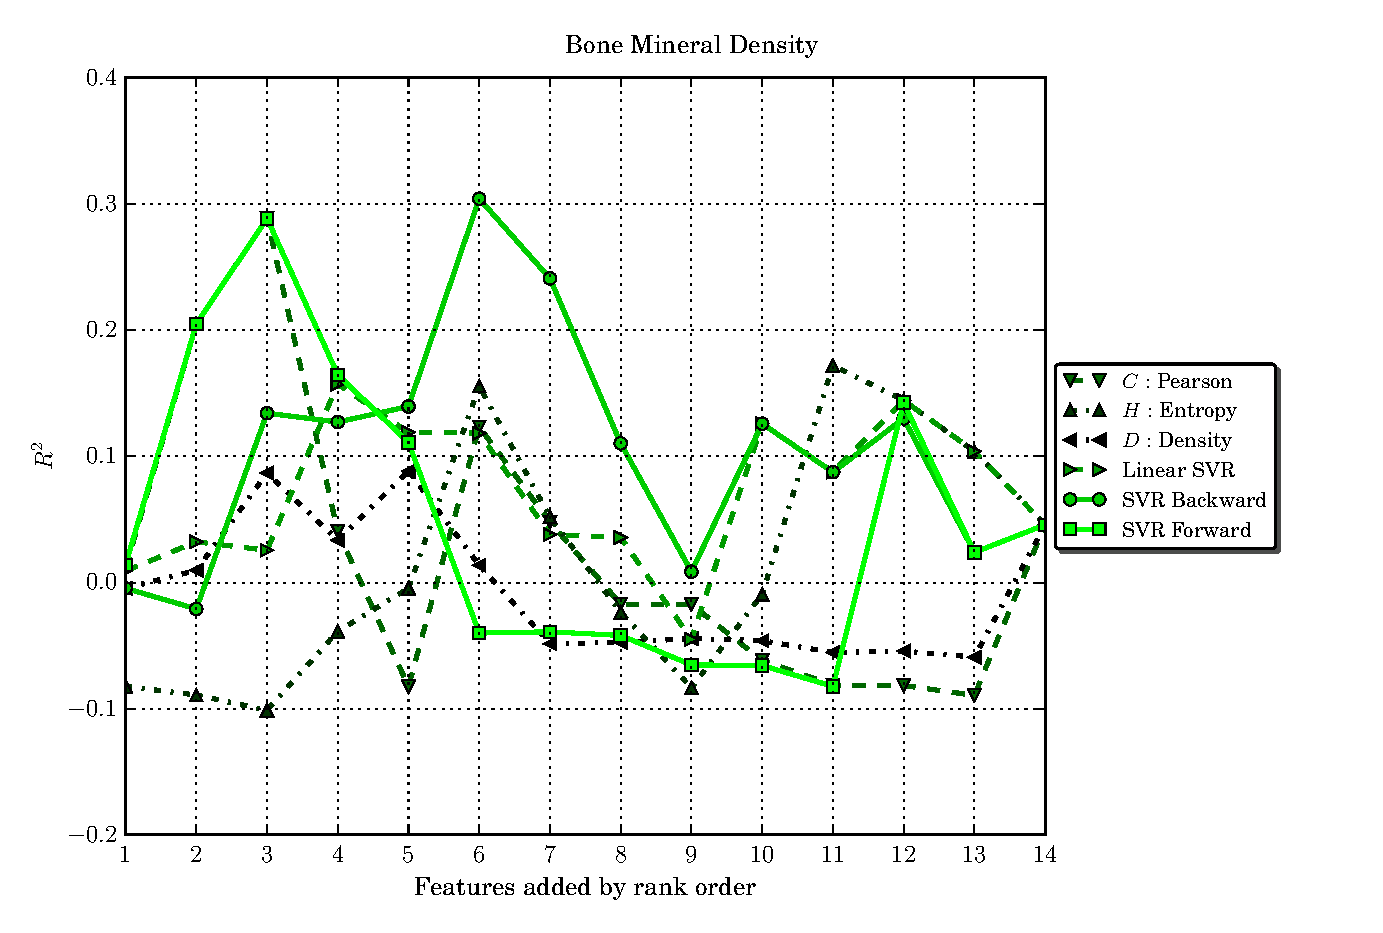
\includegraphics[width=\textwidth]{bmd_r2.eps}
\end{figure}
The figure plots all $\mathbf{e}$ vectors starting from one feature to all 14.
Note that since the first feature added, \emph{i.e.}, the best, is distinct for every
method, the initial score varies. However, all converge to the same score once
all 14 features are considered together. Ideally, we want the set of features
that achieves the highest scores with the smallest number of features. From the 
figure we observe that the best relevance feature ranking strategies are
Pearson correlation coefficient, $C$, SVR forward, and SVR backward.
Particularly, SVR forward and Pearson correlation score high with only three
features, while SVR backward performs high with six features.

The next logical step is to analyze which features are in the set that produced
the highest score for all methods in order to determine which are more
frequent. Table \ref{tbl:bestfeats} presents a summary of which features are
frequently part of the best set of features for a given ranking methodology.
The table also presents a weighted frequency count using the rank of each
method. The rank was determined as the best overall score of a given method
regardless of the number of features. From Figure \ref{fig:results} it can be
determined that the best score corresponds to SVM backward and the worst to
Density. 

\begin{table}[t]
\caption{Analysis of sets of features producing the best score. Each column
corresponding to a ranking method has a format $b/r$, where $b$ is either a
zero or a one, indicating that the feature was part of the set that produced
the best score for that method; $r$ is the rank of that method compared to the
others. The method with the best overall score is ranked one and the worst is
ranked as six; in case of a tie, the ranks are averaged. The last column shows
the frequency count of how many times that feature was part of a best set; in
parenthesis, $w_\text{Freq.}$ indicates the sum of $r/b$ for each feature as a
weighted frequency count based on the rank. Quantities resulting in zero have
been omitted.}
      \begin{tabular}{clccccccc}
        \hline
\multirow{2}{*}{$\mathcal{F}$} & 
\multirow{2}{*}{Feature} & 
\multirow{2}{*}{$C$} &
\multirow{2}{*}{$H$} &
\multirow{2}{*}{$D$} &
Lin. &
SVR &
SVR & 
Freq. \\
   &                                 &       &       &     &  SVR & Bwd. &  Fwd. &  ($w_\text{Freq.}$) \\ \hline
1  & Drinking Category               &       &   1/4 & 1/6 &      &  1/1 &       &  3 (1.42) \\
2  & Sex                             & 1/2.5 &       & 1/6 &      &      & 1/2.5 &  3 (0.97) \\
3  & Age at First Intoxication       & 1/2.5 &   1/4 & 1/6 &      &      & 1/2.5 &  4 (1.22)\\
4  & $\mu$ of Maximum Bout Vol.      &       &   1/4 &     &  1/5 &  1/1 &       &  3 (1.45)\\
5  & $\sigma$ of Maximum Bout Vol.   &       &   1/4 &     &  1/5 &  1/1 &       &  3 (1.45)\\
6  & Median of Maximum Bout Vol.     & 1/2.5 &   1/4 &     &  1/5 &  1/1 & 1/2.5 &  5 (2.25)\\
7  & $\max$ of Maximum Bout Vol.     &       &   1/4 &     &      &      &       &  1 (0.25)\\
8  & $\min$ of Maximum Bout Vol.     &       &   1/4 & 1/6 &      &      &       &  2 (0.42)\\
9  & $\mu$ \% of EtOh During Ind.    &       &   1/4 &     &      &  1/1 &       &  2 (1.25)\\
10 & Median \% of EtOh During Ind.   &       &       &     &      &      &       &   \\
11 & $\Sigma$ \% of EtOh During Ind. &       &   1/4 &     &  1/5 &  1/1 &       &  3 (1.45) \\
12 & $\sigma$ \% of EtOh During Ind. &       &   1/4 &     &      &      &       &  1 (0.25)\\
13 & $\min$ \% of EtOh During Ind.   &       &   1/4 &     &      &      &       &  1 (0.25)\\ 
14 & $\max$ \% of EtOh During Ind.   &       &       & 1/6 &      &      &       &  1 (0.17)\\ \hline
      \end{tabular}
\label{tbl:bestfeats}
\end{table}

Careful inspection of Table \ref{tbl:bestfeats} reveals that, considering the
frequency count of the features, the two features that are frequently part of
the best sets of features are, (with a count of 5) median of maximum bout 
volume and (with a count of 4) age at
first intoxication. On the other hand, if we consider the weighted frequency
count which ponders the count using the rank, we observe that the top two
features are, again, median of maximum bout volume with $w_\text{Freq.}=2.25$,
and three ties with $w_\text{Freq.}=1.45$ for $\mu$ of maximum bout volume, 
$\sigma$ of maximum bout volume, and $\Sigma$ \% of EtOh during induction.

In a general sense, Table \ref{tbl:bestfeats} suggests that features 
related to drinking patterns are associated
with the information of age at onset of intoxication in predicting BMD.
This is consistent with the findings shown in Table \ref{tbl:ranking}.

Figure \ref{fig:maxb_age} depicts how two features, namely ``median maximum
bout volume'' and ``age at first intoxication'', interact with each other in
predicting BMD. The figure suggests that lower BMD is associated with a median
maximum bout volume between 10 and 150 mL for young monkeys whose age is 1400
and 1700 days of age. The risk of having low BMD is less for older monkeys of
ages greater thatn 2400 days. This two features do not appear to have a linear
relationship in a two-dimensional plane; however, using the kernel method in
SVRs, the possibility of having a linear relationship in a higher-dimensional space is
often assumed.

\begin{figure}[t]
    \caption{\csentence{BMD values using ``median maximum bout volume'' and 
                        ``age at first intoxication'' as predictors.}
Predicted BMD suggests that young monkeys are at higher risk of low BMDs if
their median maximum bout volume is in the range of 10 and 150 mL.}
\label{fig:maxb_age}
    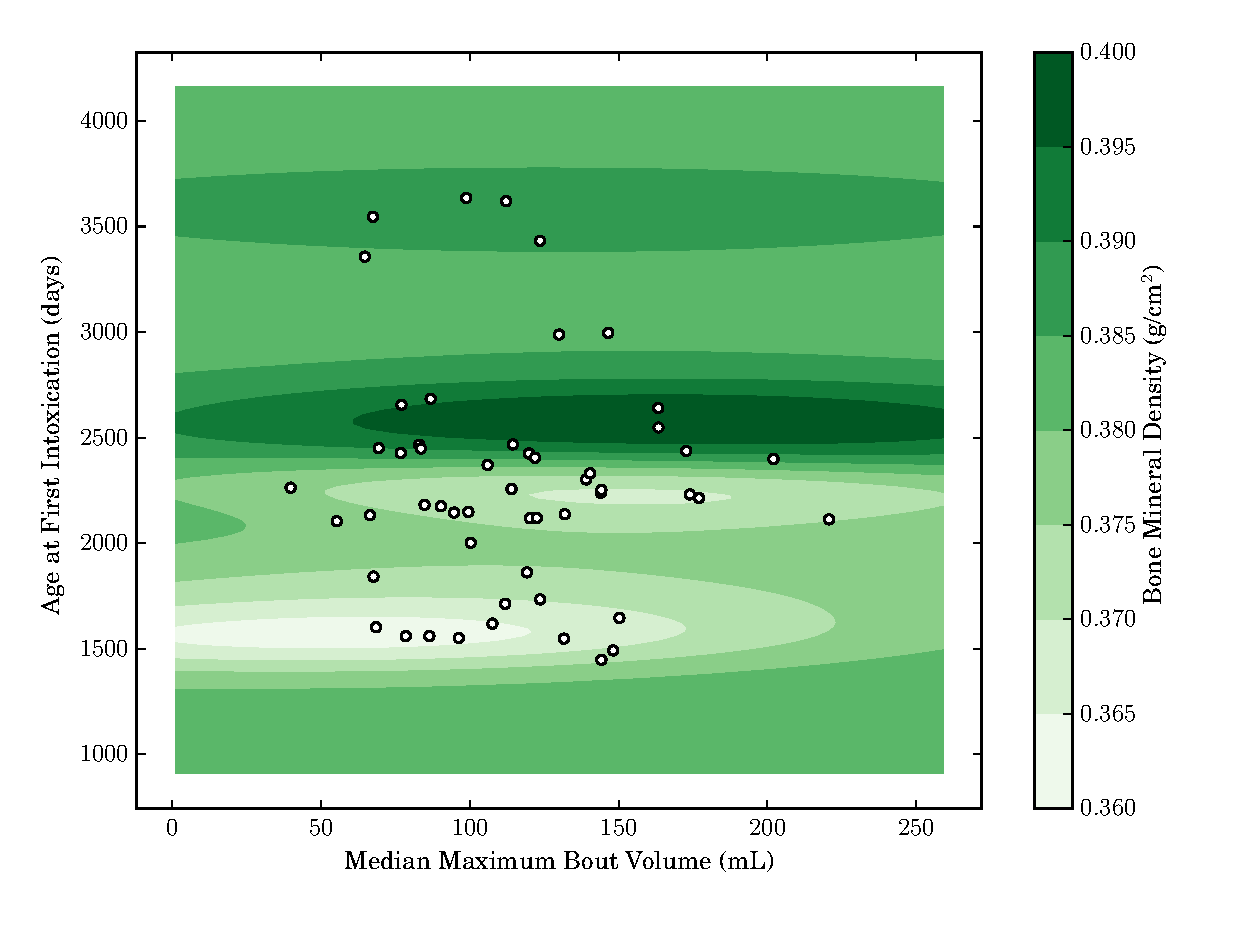
\includegraphics[width=\textwidth]{mmbv_aafi.eps}
\end{figure}

A similar analyis is shown in Figure \ref{fig:maxb_sum}. In this case the
two features analized are ``median maximum bout volume'' and ``sum of \% EtOh
during induction''. The relationship between these two features appears to be
quasi-linear, suggesting a more evident dependence or correlation. From the
figure, we can observe that if the median maximum bout volume is less than 100
mL there is a higher risk of low BMD for almost any sum of \% of EtOh, while
the risk decreases in the opposite direction.

\begin{figure}[t]
    \caption{\csentence{Performance of the sets of features using the $R^2$
                        score.}
Pearson correlation coefficient, SVR backward, and SVR forward score the
highest among all. With SVR forward and Pearson correlation coefficient the scores
are achieved with only three features, while SVR backward with six features.}
\label{fig:maxb_sum}
    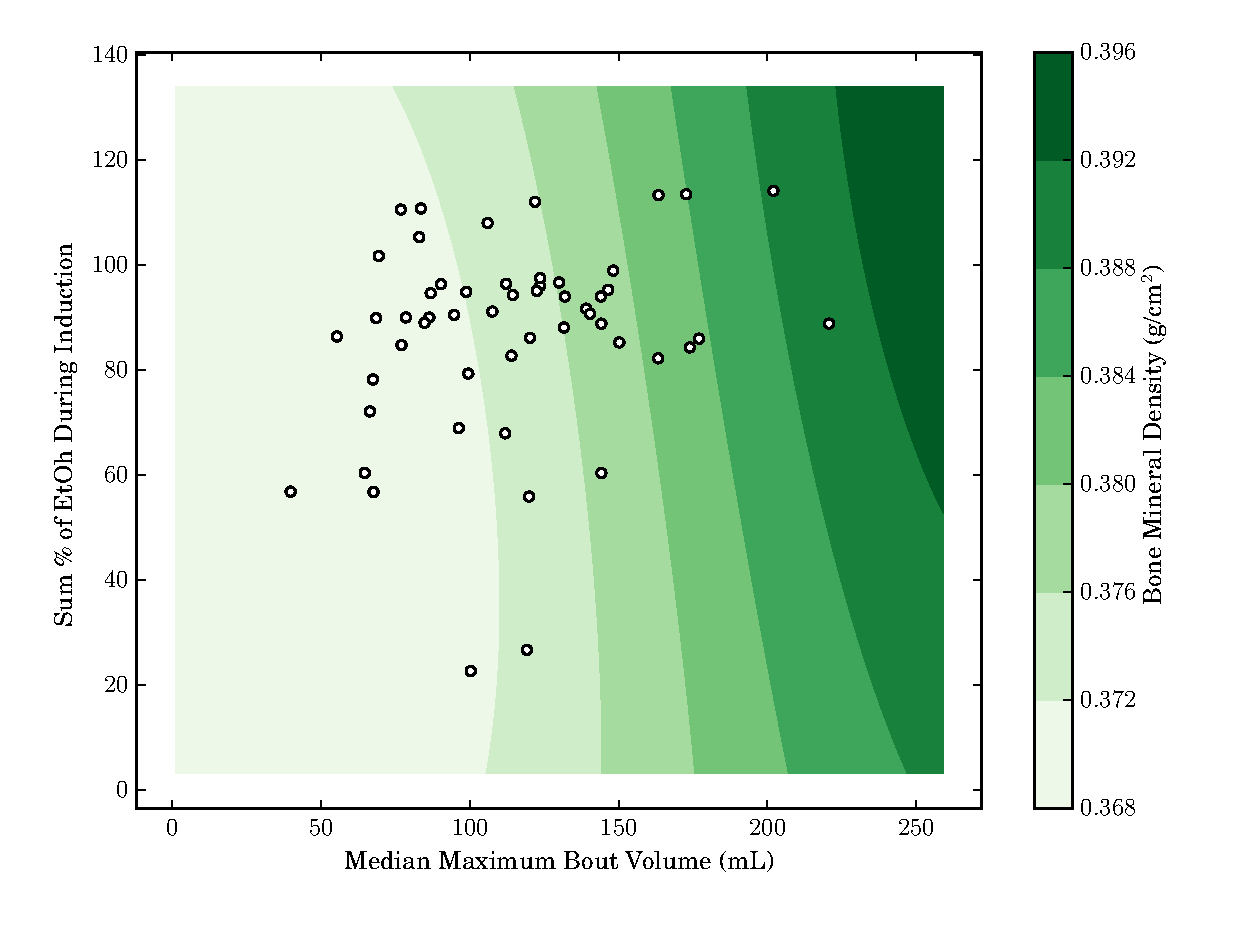
\includegraphics[width=\textwidth]{mmbv_soedi.eps}
\end{figure}

\section*{Conclusion}
Using machine learning techniques known as relevance feature ranking we
explored a dataset containing several attributes concerning drinking
patterns in primates. Such attributes were categorical and quantitative. We
determined that the ``median maximum bout volume'', ``sum of \% of EtOh during
induction'', ``$\mu$ of maximum bout volume'', ``$\sigma$ of maximum bout
volume'', and ``age at first intoxication'' are the features most predictive  
of bone mineral density.
Further analysis indicated that there are features significantly better than
others in a statistical sense; this was later demonstrated, also, through a full
training of SVRs over the data, adding features as they were ranked by each
method.

We also analyzed the complexity of the feature ranking algorithms and observed
that the Pearson correlation coefficient is significantly less expensive and
performs well for very up to three features, after that, Pearson does not
consider the interdependence of the data. On the other hand, the SVR Backward
selection strategy was the best of all, considering all the features at once
and their relationship as a group; however, it is more expensive than Pearson's
coefficient.




%%%%%%%%%%%%%%%%%%%%%%%%%%%%%%%%%%%%%%%%%%%%%%
%%                                          %%
%% Backmatter begins here                   %%
%%                                          %%
%%%%%%%%%%%%%%%%%%%%%%%%%%%%%%%%%%%%%%%%%%%%%%

\begin{backmatter}

\section*{Competing interests}
  The authors declare that they have no competing interests.

\section*{Author's contributions}
PRP designed and performed the relevance feature ranking study. All authors were
actively involved in the project. EB provided data and experimental design. UI and KG provided the data. PRP conducted the 
analysis. EB, UI and KG revised early drafts of the manuscript. All
authors commented on and approved the final version of the manuscript.

\section*{Acknowledgements}
This work was supported by NIAAA grant AA019431.
This work was supported in part by the National Council for Science and
Technology (CONACyT), Mexico, under grant 193324/303732 provided to PRP.

%%%%%%%%%%%%%%%%%%%%%%%%%%%%%%%%%%%%%%%%%%%%%%%%%%%%%%%%%%%%%
%%                  The Bibliography                       %%
%%                                                         %%
%%  Bmc_mathpys.bst  will be used to                       %%
%%  create a .BBL file for submission.                     %%
%%  After submission of the .TEX file,                     %%
%%  you will be prompted to submit your .BBL file.         %%
%%                                                         %%
%%                                                         %%
%%  Note that the displayed Bibliography will not          %%
%%  necessarily be rendered by Latex exactly as specified  %%
%%  in the online Instructions for Authors.                %%
%%                                                         %%
%%%%%%%%%%%%%%%%%%%%%%%%%%%%%%%%%%%%%%%%%%%%%%%%%%%%%%%%%%%%%

% if your bibliography is in bibtex format, use those commands:
\bibliographystyle{bmc-mathphys} % Style BST file (bmc-mathphys, vancouver, spbasic).
\bibliography{rivas_bmc}      % Bibliography file (usually '*.bib' )
% for author-year bibliography (bmc-mathphys or spbasic)
% a) write to bib file (bmc-mathphys only)
% @settings{label, options="nameyear"}
% b) uncomment next line
%\nocite{label}

% or include bibliography directly:
% \begin{thebibliography}
% \bibitem{b1}
% \end{thebibliography}

%%%%%%%%%%%%%%%%%%%%%%%%%%%%%%%%%%%
%%                               %%
%% Figures                       %%
%%                               %%
%% NB: this is for captions and  %%
%% Titles. All graphics must be  %%
%% submitted separately and NOT  %%
%% included in the Tex document  %%
%%                               %%
%%%%%%%%%%%%%%%%%%%%%%%%%%%%%%%%%%%

%%
%% Do not use \listoffigures as most will included as separate files

%% \section*{Figures}
%%   \begin{figure}[h!]
%%   \caption{\csentence{Sample figure title.}
%%       A short description of the figure content
%%       should go here.}
%%       \end{figure}
%% 
%% \begin{figure}[h!]
%%   \caption{\csentence{Sample figure title.}
%%       Figure legend text.}
%%       \end{figure}

%%%%%%%%%%%%%%%%%%%%%%%%%%%%%%%%%%%
%%                               %%
%% Tables                        %%
%%                               %%
%%%%%%%%%%%%%%%%%%%%%%%%%%%%%%%%%%%

%% Use of \listoftables is discouraged.
%%
%% \section*{Tables}
%% \begin{table}[h!]
%% \caption{Sample table title. This is where the description of the table should go.}
%%       \begin{tabular}{cccc}
%%         \hline
%%            & B1  &B2   & B3\\ \hline
%%         A1 & 0.1 & 0.2 & 0.3\\
%%         A2 & ... & ..  & .\\
%%         A3 & ..  & .   & .\\ \hline
%%       \end{tabular}
%% \end{table}

%%%%%%%%%%%%%%%%%%%%%%%%%%%%%%%%%%%
%%                               %%
%% Additional Files              %%
%%                               %%
%%%%%%%%%%%%%%%%%%%%%%%%%%%%%%%%%%%

%% \section*{Additional Files}
%%   \subsection*{Additional file 1 --- Sample additional file title}
%%     Additional file descriptions text (including details of how to
%%     view the file, if it is in a non-standard format or the file extension).  This might
%%     refer to a multi-page table or a figure.
%% 
%%   \subsection*{Additional file 2 --- Sample additional file title}
%%     Additional file descriptions text.


\end{backmatter}
\end{document}
